\documentclass[oneside,a4paper,14pt]{extarticle}
\usepackage[a4paper,top=20mm,bottom=20mm,left=30mm,right=10mm]{geometry}
\usepackage{amsmath, amssymb, amsfonts, amsthm}
\usepackage[T2A]{fontenc}
\usepackage[utf8]{inputenc}
\usepackage[russian]{babel}
\usepackage{textcomp}
\usepackage{indentfirst}
\usepackage{graphicx}
\usepackage{float}
\usepackage{wrapfig}
\usepackage{caption}
\usepackage{tocloft}
\usepackage{seqsplit}
\allowbreak
\renewcommand{\cftsecleader}{\cftdotfill{\cftdotsep}}
\usepackage[breaklinks]{hyperref}
\usepackage{titlesec}
\usepackage{fancyvrb}
\usepackage{xcolor}
\titleformat{\section}{\normalsize\bfseries}{\thesection}{1em}{}
\titleformat{\subsection}{\normalsize\bfseries}{\thesubsection}{1em}{}
\titleformat{\subsubsection}{\normalsize\bfseries}{\thesubsubsection}{1em}{}
\renewcommand\baselinestretch{1.33}\normalsize
\setlength{\parindent}{1.25cm}

\captionsetup[figure]{labelsep=period}

\begin{document}
\newpage\thispagestyle{empty}
\newpage
\setcounter{page}{1}
\tableofcontents
\newpage

\section*{Задание}
\addcontentsline{toc}{section}{Задание}
Задание для шестого варианта:\\
Микрооперации:
\begin{enumerate}
	\item Суммирование двух 8-разрядных двоичных чисел в дополнительном коде (содержащих в старшем (седьмом) разряде знак числа).
	\item Циклический сдвиг 8-разрядного двоичного числа на один разряд в сторону младших разрядов.
\end{enumerate}
Логические условия:
\begin{enumerate}
	\item S - знак результата.
	\item OVR - признак переполнения.
\end{enumerate}
\section*{Анализ задания по разработке функциональной модели}
\addcontentsline{toc}{section}{Анализ задания по разработке функциональной модели}

Разрабатываемая функциональная модель будет иметь три 8-разрядных входа операндов (X1, X2 и Y), а также 8-разрядный выход результата (Z) и одноразрядные выходы признаков: – знак результата (S) и переполнения (OVR).

\newpage\section*{Описание работы узла с помощью системы булевых функций}
\addcontentsline{toc}{section}{Описание работы узла с помощью системы булевых функций}

АЛБ имеет три информационных входа, на которые могут поступать исходные данные: на первый вход двоичный 8-разрядный код\\
$X_1=x_7x_6x_5x_4x_3x_2x_1x_0$, на второй - $X_2=x_7x_6x_5x_4x_3x_2x_1x_0$, а также вход $Y=y_7y_6y_5y_4y_3y_2y_1y_0$. Узел имеет один информационный выход, где формируется результат: 8-разрядный двоичный код
$Z=z_7z_6z_5z_4z_3z_2z_1z_0$.

Управляющие сигналы и выполняемые микрооперации:\\
$ v_2 $ - суммирование двух 8-разрядных двоичных чисел в дополнительном коде: $A=X_1+X_2$;\\
$ v_1 $ - циклический сдвиг 8-разрядного двоичного числа на один разряд в сторону младших разрядов.\\

Выполнение микрооперации осуществляется при единичном значении соответствующего управляющего сигнала p0. Сигнал $k_0$ задаёт перенос в младший разряд при суммировании.

Микрооперации и логические условия можно описать следующими системами булевых функций.

\subsection*{Суммирование в дополнительном коде}

Для $n=1,\dots,8$:
\[
	a_{n-1}=v_2\&(x_{n-1}\oplus y_{n-1}\oplus p_{n-1}),
\]
\[
	p_n=v_2\&(x_{n-1}\&y_{n-1}\vee x_{n-1}\&p_{n-1}\vee y_{n-1}\&p_{n-1}).
\]

При этом $p_0=1$ или $p_0=0$ в зависимости от режима суммирования.

Признак переполнения при суммировании в дополнительном коде:
\[
	OVR=p_8\oplus p_7.
\]
\newpage
\subsection*{Циклический сдвиг в сторону младших разрядов}

При $v_1=1$:
\[
	b_{n}=v_1\&y_{n+1}, \quad n=0,\dots,6,
\]
\[
	b_7=v_1\&y_0.
\]

Разряды результата сдвига формируются следующим образом:
\[
	b_0=y_1,\quad b_1=y_2,\quad \dots,\quad b_6=y_7,\quad b_7=y_0.
\]

\subsection*{Результат на выходе АЛБ}

\[
	z_{n-1}=a_{n-1}\vee b_{n-1}, \quad n=1,\dots,8.
\]

Знак результата:
\[
	S=z_7.
\]

\section*{Разработка схемы блока}
\addcontentsline{toc}{section}{Разработка схемы блока}

На основе системы булевых функций АЛБ может быть построена схема, описывающая его функционирование, она представлена на рис.1. АЛБ содержит две основные логические схемы микроопераций:

\begin{itemize}
	\item \textbf{LS0} - суммирование $X_1+X_2$ в дополнительном коде;
	\item \textbf{LS1} - циклический сдвиг в сторону младших разрядов.
\end{itemize}

Также имеется вспомогательная логическая схема \textbf{LS2} <<A $\vee$ B>>, которая позволяет выдавать результат выполняемой микрооперации на выход $Z$ АЛБ.

На логические схемы микроопераций LS0 и LS1 кроме исходных данных поступает соответствующий управляющий сигнал ($v_2$ или $v_1$). На схему суммирования также поступает сигнал переноса в младший разряд $k_0$. Выдачу на выход признака переполнения $OVR$ обеспечивает логический элемент, формирующий сигнал переполнения при суммировании в дополнительном коде. На выходе $S$ формируется знак результата - старший разряд $z_7$.

\section*{Разработка экранной формы для экспериментального исследования блока}
\addcontentsline{toc}{section}{Разработка экранной формы для экспериментального исследования блока}

Пример экранной формы для исследования АЛБ показан на рис.1. В верхней части экранной формы расположены два 8-разрядных поля ввода исходных данных $X_1$ и $X_2$, а также поле для ввода числа $Y$, над которым выполняется циклический сдвиг. На экранной форме расположены одноразрядные поля для ввода управляющих сигналов ($v_1$, $v_2$) и сигнала переноса в младший разряд $k_0$.

Микрооперации представлены на экранной форме логическими схемами (LS0, LS1, LS2), на которых отображаются 8-разрядные поля вычисляемых результатов. На сумматоре LS0 кроме вычисленной суммы дополнительно отображается 8-разрядное слово переносов. В нижней части экранной формы показан информационный выход, где формируется результат: 8-разрядный двоичный код $Z$. В левой части экранной формы отображаются признаки: знак результата $S$ и признак переполнения $OVR$.

\begin{figure}[H]
	\centering
	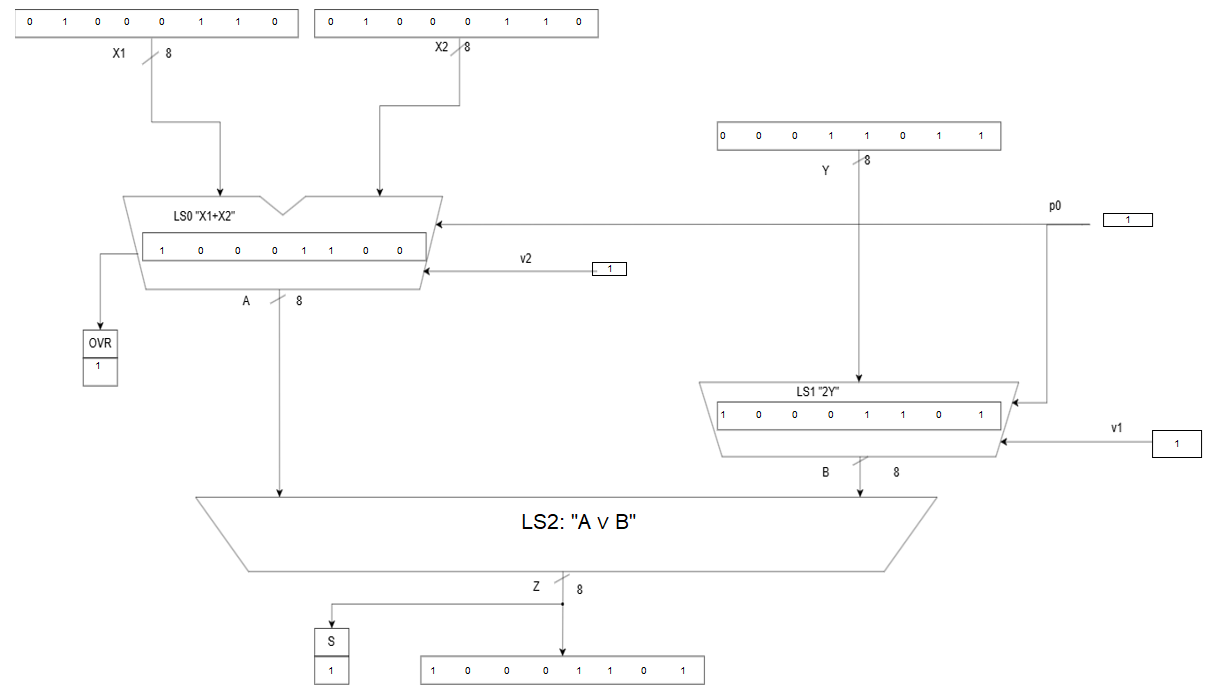
\includegraphics[width=0.95\textwidth]{Полная схема.png}
	\caption{Экранная форма для исследования АЛБ}
	\label{fig:als}
\end{figure}

\section*{Построение функциональной модели блока}
\addcontentsline{toc}{section}{Построение функциональной модели блока}

Работа АЛБ моделируется путём реализации формул булевых функций с помощью логических функций табличного процессора MS Excel. Реализация формул булевых функций показана в табл.1. Ввиду однотипности формул, соответствующих отдельным разрядам, в таблице для всех микроопераций приводятся формулы для младшего разряда, а для суммирования - ещё и для старшего разряда результата.

\begin{flushright}
	Таблица 1
\end{flushright}
\begin{center}
	Реализация формул булевых функций\\
\end{center}
\begin{small}
	\begin{tabular}{|p{5.6cm}|p{1.8cm}|p{8.6cm}|}
		\hline
		Микрооперация / Формула булевой функции         & Адрес ячейки & Формула                                                              \\
		\hline
		Суммирование                                    &              &                                                                      \\
		\hline
		$a_0=v_2\&(x_0\oplus y_0\oplus p_0)$            & F18          & \texttt{=ЕСЛИ(AND(S19;AF16);       ЕСЛИ(XOR(E109;A113);1;0);0)}      \\
		\hline
		$p_1=v_2\&(x_0\&y_0\vee x_0\&p_0\vee y_0\&p_0)$ & W30          & \texttt{=ЕСЛИ(ИЛИ(И(E109;A113);       И(E109;AL5);И(A113;AL5));1;0)} \\
		\hline
		$a_7=v_2\&(x_7\oplus y_7\oplus p_7)$            & M8           & \texttt{=ЕСЛИ(AND(S19;AF16);      ЕСЛИ(XOR(B79;A82);1;0);0)}         \\
		\hline
		$p_8=v_2\&(x_7\&y_7\vee x_7\&p_7\vee y_7\&p_7)$ & AC30         & \texttt{=ЕСЛИ(ИЛИ(И(B79;A82);        И(B79;AC30);И(A82;AC30));1;0)}  \\
		\hline
		Циклический сдвиг                               &              &                                                                      \\
		\hline
		$b_0=v_1\&y_1$                                  & F18          & \texttt{=IF(AF16;IF(лаба1!AG31;V10;W10);0)}                          \\
		\hline
		$b_6=v_1\&y_7$                                  & L8           & \texttt{=IF(AF16;IF(лаба1!AG31;AA10;AB10);0)}                        \\
		\hline
		$b_7=v_1\&y_0$                                  & M8           & \texttt{=IF(AF16;IF(лаба1!AG31;AC10;V10);0)}                         \\
		\hline
		Результат                                       &              &                                                                      \\
		\hline
		$z_0=a_0\vee b_0$                               & F18          & \texttt{=ЕСЛИ(ИЛИ(F18;F18);1;0)}                                     \\
		\hline
		$z_7=a_7\vee b_7$                               & M8           & \texttt{=ЕСЛИ(ИЛИ(M8;M8);1;0)}                                       \\
		\hline
		Признак $S$                                     & S            & \texttt{=M8}                                                         \\
		\hline
		Признак $OVR$                                   & OVR          & \texttt{=ЕСЛИ(ИСКЛИЛИ(AC30;AB30);1;0)}                               \\
		\hline
	\end{tabular}
\end{small}
\newpage
\section*{Экспериментальные исследования функциональной модели блока}
\addcontentsline{toc}{section}{Экспериментальные исследования функциональной модели блока}

В процессе экспериментальных исследований осуществляется проверка правильности выполнения микроопераций и формирования логических условий. В табл.~\ref{tab:results} приведены примеры выполнения микроопераций и формирования логических условий.
\begin{flushright}
	Таблица 2
\end{flushright}
\begin{center}
	Результаты вычисления микроопераций и логических условий
\end{center}

\begin{small}
	\begin{tabular}{|c|c|c|c|c|c|c|c|c|}
		\hline
		$p_0$ & $v_2$ & $v_1$ & МО                & $X_1$    & $X_2$ / $Y$ & $W$      & $S$ & $OVR$ \\
		\hline
		1     & 1     & 0     & Суммирование      & 10001001 & 00001111    & 10011000 & 1   & 0     \\
		\hline
		1     & 1     & 0     & Суммирование      & 01111111 & 00000001    & 10000000 & 1   & 1     \\
		\hline
		1     & 1     & 0     & Суммирование      & 11111111 & 11111111    & 11111110 & 1   & 0     \\
		\hline
		1     & 0     & 0     & Суммирование      & 11111111 & 11111111    & 00000000 & 0   & 0     \\

		\hline
		1     & 0     & 1     & Циклический сдвиг & -        & 10000001    & 11000000 & 1   & -     \\
		\hline
		1     & 0     & 1     & Циклический сдвиг & -        & 00000011    & 10000001 & 1   & -     \\
		\hline
		0     & 0     & 1     & Циклический сдвиг & -        & 10000001    & 00000000 & 0   & -     \\
		\hline
		1     & 0     & 0     & Циклический сдвиг & -        & 11111110    & 00000000 & 0   & -     \\

		\hline
	\end{tabular}
\end{small}\\

В таблице суммирование исходных чисел $X_1=10001001$ и $X_2=00001111$ произведено с помощью сумматора (строка 1). При этом результат равен $10011000$, знак результата $S=1$, переполнение $OVR=0$.

В строке 2 приведён пример переполнения: $X_1=01111111$, $X_2=00000001$, результат $10000000$, $S=1$, $OVR=1$. Это соответствует ситуации, когда сумма двух положительных чисел в дополнительном коде даёт отрицательный результат.

В строке 3 показано суммирование двух отрицательных чисел: $X_1=11111111$, $X_2=11111111$, результат $11111110$, $S=1$, $OVR=0$.

Строки 4--6 иллюстрируют работу циклического сдвига в сторону младших разрядов. Например, при $Y=10000001$ результат равен $11000000$, то есть младший разряд $y_0=1$ переносится в старший разряд $z_7$, а остальные разряды сдвигаются вправо. При $Y=00000011$ результат равен $10000001$. При $Y=00000000$ результат также равен $00000000$, признак $Z=1$.
\newpage
\section*{Вывод}
\addcontentsline{toc}{section}{Вывод}

В ходе выполнения лабораторной работы была разработана схема булевых функций, описывающая работу арифметико-логического блока для суммирования двух 8-разрядных двоичных чисел в дополнительном коде и циклического сдвига 8-разрядного двоичного числа на один разряд в сторону младших разрядов. На основе схемы булевых функций были составлены их представления в MS Excel и построена экранная форма узла для экспериментального исследования. В ходе экспериментального исследования составлена таблица результатов, которая отражает работу узла без ошибок. Признаки $S$ и $OVR$ формируются корректно, что подтверждает правильность построенной функциональной модели.

\end{document}